% !TEX root = ./thesis.tex

\chapter{Model}

In this chapter we provide overview of our method.
First we provide details about our model initialization and training procedure.
Than we describe baseline architectures that we used as the backbone of our model during evaluation.
At last, we describe our method of robust manifold learning.


\label{ch:mode}

\section{Training process}

In our traingin we use a server with Intel Xeon CPU 2.40GHz, 64GB of RAM and a GeForce GTX TITAN X Kepler graphics card with 12GB of video memory. Server runs Debian 8.7 operation system with CUDA 8.0, CuDNN 5.1 and TensorFlow 1.0 installed.

\subsection{Tensorflow}

In deep learning TensorFlow \cite{GoogleResearch2015, Abadi2016}, Torch \cite{torch}, and Caffe \cite{jia2014caffe} are among the most common choices of scientific computing framework.
These frameworks use different underlying programming languages and show different compatibility features and qualities of managing computational resources.

We use TensorFlow as our scientific computing framework of choice.

TensorFlow is an open source cross platform software library.
TensorFlow constructs complex computational procedures in form of computational graphs.
Nodes of the computational graph represent some mathematical operations.
Edges of the graph represent data flow between nodes in form of multidimensional arrays, also called tensors.

\begin{figure}[h!]
  \centering
    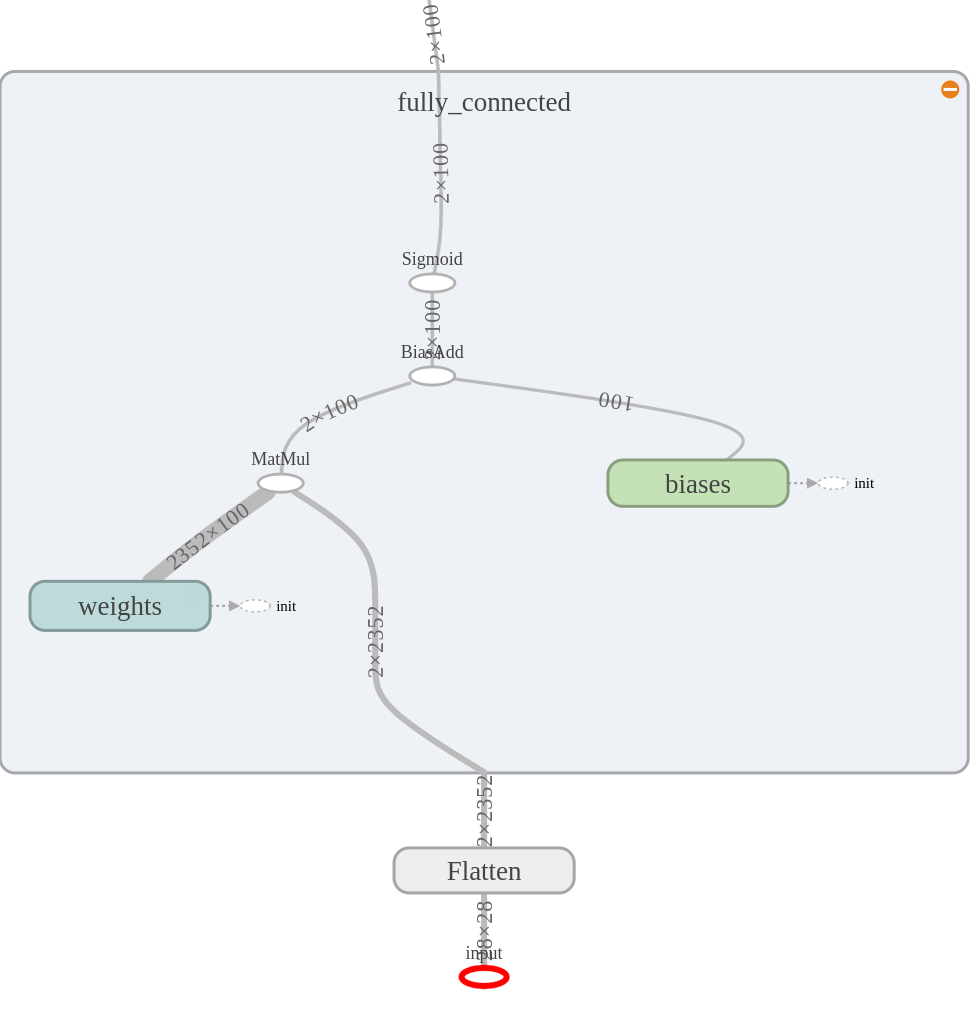
\includegraphics[width=0.7\textwidth,height=0.7\textheight,keepaspectratio]{tf_graph_1.png}
  \caption{TensorFlow detailed graph representation of a single fully connected layer with 100 neurons and sigmioid activation function. Image produced with the build in visualization tool.}
  \label{fig:tf_graph}
\end{figure}

TensorFlow provides cross platform compatiblity, which allows to run code on defferent types of devices and operation systems.
Abstraction over underlying system allows to run models, build with TensorFlow, both on GPUs and CPU without code changes.
Integration with hight performance computing libraries as CUDA \cite{Nickolls2008} and native support of distributed computing makes it a good candidate for computer vision tasks.
An competition winning family of convolutional neural networks Inception is solely developed and maintained on that platform \cite{Szegedy2016}.

We use TensorFlow as our framework of choice for several reasons.
First of all, being a crossplatform frameworks it enables larger audience to reuse results of our research.
Second, it allows to easily configure and run deep network architecture and, at the same time, apply non-trivial modification to the computational flow.
And, at last, it provides build-in visualization tools that allow better control of the leraning process.

All our code is shared for public use under MIT License.
\footnote{\url{https://github.com/yselivonchyk/TensorFlow_DCIGN}}

\subsection{Training algorithm}

We run the training using stochastic gradient descent algorihtm with mini-batches \ref{alg:bp}. We use adaptive learning rate in form of Adam update rule \ref{alg:adam}. Adaptive learning rate rule has shown to lead to convergence of the backpropagation algorithm at least as often as other methods. It also showed to converge consistently even for a single learning rate for different models.

We use mini-batch size of 128 as the largest one that fits into video memory for each model.
We also found that gradient descent convergice for each of the tested models with lerning rate $\nu=0.0001$ is used. This learning rate falls into the interval of recommended learning rates for Adam update rule \cite{Kingma2015}.

We use early stopping as the termination condition of the algorithm \ref{alg:bp}.

To select hyperparameters of the model, such as weights $\alpha, \beta$ of a composite error $L=L_1 + \alpha L_2 + \beta L_3$, layer sizes etc. we perform a single grid search per parameter.
Grid search is executed for a single parameter at a time, while other parameters stay fixed.
In each grid search is performed for 3 values $\{p_1, p_2, p_3\}$. Whenever better results are achieved for border values $p_1$ or $p_3$, the grid is shifted in the direction of the winning value. When middle value $p_2$ shows the best result but the difference is significant grid search is repeated for decreased grid size.
When parameter shows no effect on model performance the value, that causes better computational efficiency of the model, is selected.

\subsection{Model parameter initialization}

Initial model parameters $\theta$ in conjunction with learning algorithm play crucial role in finding good local minima of optimization problem.
Gradient descent algorithm does not guarantee convergence in finite number of steps.
Hence, model parameters can stay in a "noisy" region where, regardless of learning rate, step in the direction of the gradient on average causes zero decrease of the loss.

It has been shown, that bad weight initialization can lead to exploding or diying out signal especially in deep architectures \cite{Glorot2010}. More specifically, for very small initial weigths signal propagating to the further layers becomes too small to be useful and vise versa.
Too large and too small preactivation values can lead to saturation of sigmoid or tangent units and to dying out of ReLU units. This effectively decreases number of learning units in the network and can impeade training.

Most commonly, \textit{Xavier initialization} is used with deep neural networks to avoid situation as described above \cite{Glorot2010}.
Another options might include layer-wise weight initialization, pretraining of the parts of the model \cite{Simonyan2015} or applying weight regularization \cite{Good2016}.
Yet, we would prefer the issue of weight initialization not to effect the training process.


Xavier initializer suggest using normalized initialization, that depends on the number of inputs and ouputs of the layer \cite{Good2016}. Weight values are drown uniformly at random from a normal distribution $\Bbb{U}$:

\begin{equation}\label{eq:xavier}
  w_{j, i} \sim \Bbb{U}(
  \mu=-\frac{\sqrt{6}}{\sqrt{n_j+n_{j+1}}},
  \sigma=\frac{\sqrt{6}}{\sqrt{n_j+n_{j+1}}})
\end{equation}

where $i\in\{0, \ldots, |W_j|\}$ is a index of a weight in layer $j$ and $n_j$ is a number of input units of the layer $j$.



\section{Backbone architectures}
\subsection{Fully connected autoencoder}
\subsection{Convolutional autoencoder}
\cite{Nair2010}
\subsection{WhatWhere autoencoder}

\section{Model pretraining}



\section{Manifold learning}
\subsection{Predictive objective}
\subsection{Denoising regularization}
\subsection{Feature set regularization}
